%%%%%%%%%%%%%%%%%%%%%%%%%%%%%%%%%%%%%%%%%%%%%%%%%%%%%%%%%%%%%%%%%%%%%%%%%%%%%%%%%%%%
% Document data
%%%%%%%%%%%%%%%%%%%%%%%%%%%%%%%%%%%%%%%%%%%%%%%%%%%%%%%%%%%%%%%%%%%%%%%%%%%%%%%%%%%%
\documentclass[12pt]{report} %report allows for chapters
\renewcommand\thesection{\arabic{section}} % ignore the title number for sections
%%%%%%%%%%%%%%%%%%%%%%%%%%%%%%%%%%%%%%%%%%%%%%%%%%%%%%%%%%%%%%%%%%%%%%%%%%%%%%%%%%%%




%%%%%%%%%%%%%%%%%%%%%%%%%%%%%%%%%%%%%%%%%%%%%%%%%%%%%%%%%%%%%%%%%%%%%%%%%%%%%%%%%%%%
% Packages
%%%%%%%%%%%%%%%%%%%%%%%%%%%%%%%%%%%%%%%%%%%%%%%%%%%%%%%%%%%%%%%%%%%%%%%%%%%%%%%%%%%%
\usepackage{color, soul, xcolor} % Colored text and highlighting, respectively

%Tikz
\usepackage{tikz-cd} % For commutative diagrams
\usepackage{tikz-3dplot}
\RequirePackage{pgfplots}
\usetikzlibrary{shadows}
\usetikzlibrary{shapes}
\usetikzlibrary{decorations}
\usetikzlibrary{arrows,decorations.markings} 
\usetikzlibrary{quotes,angles}

\usepackage{mathtools}
\usepackage{answers}
\usepackage{setspace}
\usepackage{graphicx}
\usepackage{enumerate}
\usepackage{multicol}
\usepackage{mathrsfs}
\usepackage[margin=1in]{geometry} 
\usepackage{amsmath,amsthm,amssymb}
\usepackage{marvosym,wasysym} %fucking smileys
\usepackage{float}
\usepackage{morefloats}
%%%%%%%%%%%%%%%%%%%%%%%%%%%%%%%%%%%%%%%%%%%%%%%%%%%%%%%%%%%%%%%%%%%%%%%%%%%%%%%%%%%%




%%%%%%%%%%%%%%%%%%%%%%%%%%%%%%%%%%%%%%%%%%%%%%%%%%%%%%%%%%%%%%%%%%%%%%%%%%%%%%%%%%%%
% Shortcuts
%%%%%%%%%%%%%%%%%%%%%%%%%%%%%%%%%%%%%%%%%%%%%%%%%%%%%%%%%%%%%%%%%%%%%%%%%%%%%%%%%%%%
% Number systems
\newcommand{\N}{\mathbb{N}}
\newcommand{\Z}{\mathbb{Z}}
\newcommand{\C}{\mathbb{C}}
\newcommand{\R}{\mathbb{R}}
\newcommand{\Q}{\mathbb{Q}}

% Operators/functions
\newcommand{\id}{\mathrm{Id}}
\DeclareMathOperator{\sech}{sech}
\DeclareMathOperator{\csch}{csch}
%%%%%%%%%%%%%%%%%%%%%%%%%%%%%%%%%%%%%%%%%%%%%%%%%%%%%%%%%%%%%%%%%%%%%%%%%%%%%%%%%%%%




%%%%%%%%%%%%%%%%%%%%%%%%%%%%%%%%%%%%%%%%%%%%%%%%%%%%%%%%%%%%%%%%%%%%%%%%%%%%%%%%%%%%
% Environments
%%%%%%%%%%%%%%%%%%%%%%%%%%%%%%%%%%%%%%%%%%%%%%%%%%%%%%%%%%%%%%%%%%%%%%%%%%%%%%%%%%%%
% Italic font
\newtheorem{theorem}{Theorem}[section]
\newtheorem{lemma}{Lemma}[section]
\newtheorem{corollary}{Corollary}[section]
\newtheorem{axiom}{Axiom}

% Plain font
\theoremstyle{definition}
\newtheorem{definition}{Definition}[section]
\newtheorem{example}{Example}[section]
\newtheorem{remark}{Remark}[section]
\newtheorem{solution}{Solution}
\newtheorem{problem}{Problem}[section]
\newtheorem{question}{Question}[section]
\newtheorem{answer}{Answer}[section]
\newtheorem{exercise}{Exercise}[section]
%%%%%%%%%%%%%%%%%%%%%%%%%%%%%%%%%%%%%%%%%%%%%%%%%%%%%%%%%%%%%%%%%%%%%%%%%%%%%%%%%%%%

\begin{document}


\begin{center}
   \textsc{\large MATH 255, Homework 6: \emph{Solutions}}\\
\end{center}
\vspace{.5cm}

\noindent\textbf{Relevant Sections:} 16.7, 10.3, 9.3, 9.5, 16.8 \\

\noindent\textbf{Problem 1.} 
\begin{enumerate}[(a)]
    \item Write the equation for a curve 
    \[
    \gamma \colon \R \to \R^3
    \] 
    satisfying:
    \begin{itemize}
    \item Starts with $\gamma(0)=(0,0,0)$.
    \item Ignoring the $z$-component, makes a spiral. (Imagine looking from above the $xy$-plane for this).
    \item Moves upward at a constant rate in the $z$-direction.
\end{itemize}
In other words, write the equation for a curve that makes a helix with increasing radius and constant ``pitch." (Note that there are many different ways you can write such a curve!)

Plot this curve that you made to verify it is correct.
    \item Find the tangent vector $\gamma'(t)$ to this curve.
    \item Find the acceleration vector $\gamma''(t)$ to this curve.
\end{enumerate}

\begin{solution}
\begin{enumerate}[(a)]
    \item Let's choose a start and end time, since this does not actually change much.  Just pick $t_0=0$ and $t_1 = 1$.  Then, ignoring the $z$-component, we want to spiral outward. We know how to move in a circle, and spiraling outward is moving in a circle whose radius is constantly increasing. So, for example, the first two components could be
\[
(t\cos(2\pi t),t\sin(2\pi t)).
\]
Note that at $t=0$ this is $(0,0)$.  Now, we want to move upward in the $z$-direction at a constant rate, which means the $z$ component should be $t$.  So we have
\[
\gamma(t) = (t\cos(2\pi t), t\sin(2\pi t), t).
\]
Here are relevant plots:
\begin{figure}[H]
    \centering
    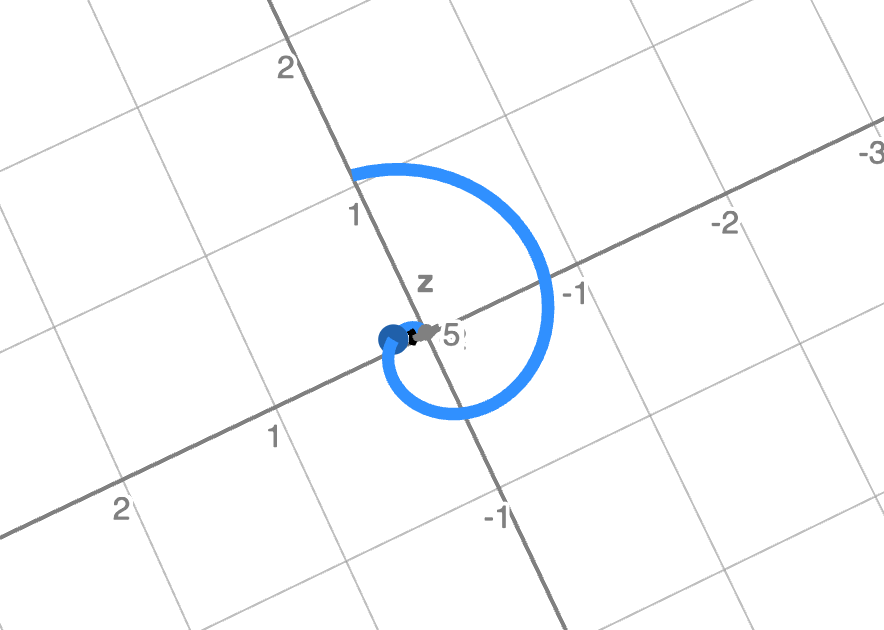
\includegraphics[width=.6\textwidth]{Images/hwk6above.png}
    \caption{A view from above.}
\end{figure}
\begin{figure}[H]
    \centering
    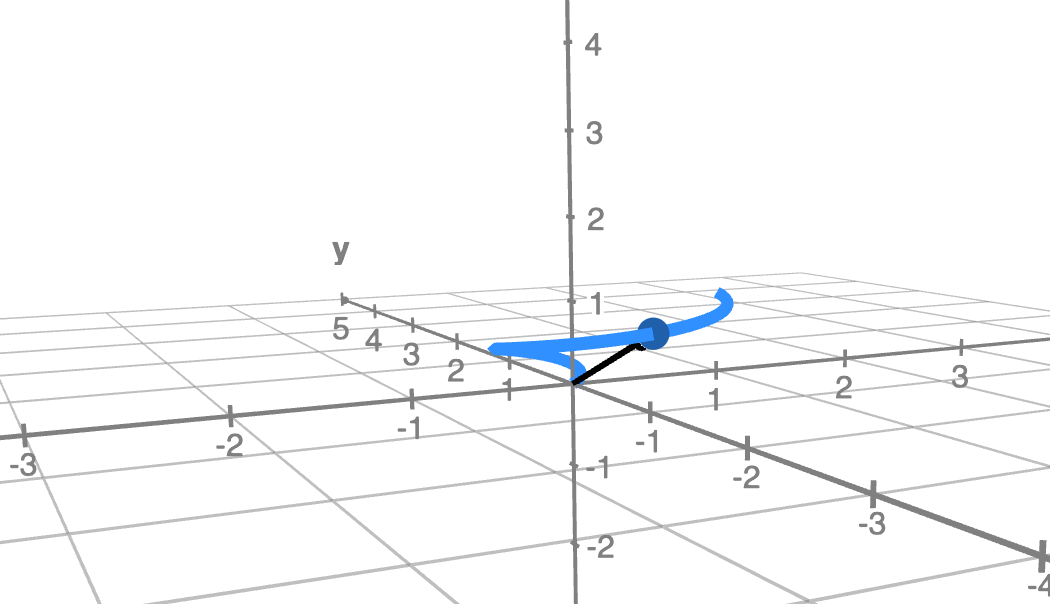
\includegraphics[width=.6\textwidth]{Images/hwk6side.png}
    \caption{A view from the side.}
\end{figure}
\item We have
\[
\gamma'(t) = (\cos(2\pi t)-2\pi t \sin(2\pi t), \sin(2\pi t) + 2\pi t \cos(2\pi t), 1).
\]
\item We have
\[
\gamma''(t) = (-4\pi(sin(2\pi t)+\pi t \cos(2\pi t)), 4\pi(\cos(2\pi t)-\pi t \sin(2\pi t),0).
\]
\end{enumerate}

\end{solution}

\noindent\textbf{Problem 2.} 
\begin{enumerate}[(a)]
    \item Write the equation for a scalar function
    \[
    f\colon \R^2 \to \R
    \]
    \begin{itemize}
        \item Has positive $\frac{\partial f}{\partial x}$ everywhere.
        \item Has negative $\frac{\partial f}{\partial y}$ everywhere.
    \end{itemize}
    (\emph{Hint: it may help to try adding single variable functions together. That is, let $f(x,y)=u(x)+v(y)$.}
    )
    \item Find the gradient of the function you chose.
\end{enumerate}
\begin{solution}~
\begin{enumerate}[(a)]
    \item I'll use the hint here since if we let
    \[
    f(x,y) = u(x)+v(y)
    \]
    then
    \[
    \frac{\partial f}{\partial x} = \frac{du}{dx}
    \]
    and
    \[
    \frac{\partial f}{\partial y} = \frac{dv}{dy}.
    \]
    This has reduced our problem to a single variable problem which we have seen before.  We want
    \begin{itemize}
        \item $\frac{\partial f}{\partial x}=\frac{du}{dx}>0$ everywhere, so we can just set $\frac{du}{dx}=1$ and integrate to find that $u(x)=x$ (really plus a constant, but that doesn't matter here).
        \item $\frac{\partial f}{\partial y}=\frac{dv}{dy}<0$ everywhere, so we can just set $\frac{dv}{dy}=-1$ and integrate to find that $v(y)=-y$.
    \end{itemize}
    So our function is
    \[
    f(x,y)=x-y.
    \]
    Note that there are many other solutions!
    
    \item We compute the gradient
    \[
    \nabla f(x,y) = \begin{bmatrix} \frac{\partial f}{\partial x} \\ \frac{\partial f}{\partial y} \end{bmatrix} = \begin{bmatrix} 1 \\ -1 \end{bmatrix}.
    \]
\end{enumerate}
\end{solution}

\noindent\textbf{Problem 3.} A rough model of a molecular crystal can be described in the following way.  Take the scalar function
\[
u(x,y)=\cos^2(x)+\cos^2(y).
\]
This function $u(x,y)$ describes the \emph{potential energy} for electrons in the crystal. Electrons are attracted to the areas with the smallest potential energy and move away from areas of high potential energy. 
\begin{enumerate}[(a)]
    \item Plot this function and include a printout.  Notice what this looks like.  You can imagine that each of the low points (well) is where a nucleus is located in the crystal.
    \item Plot the level curves where $u(x,y)=0$, $u(x,y)=\frac{1}{4}$, $u(x,y)=\frac{1}{2}$, and $u(x,y)=1$ for the range of values $-\frac{3\pi}{2}\leq x \leq \frac{3\pi}{2}$ and $-\frac{3\pi}{2}\leq y \leq \frac{3\pi}{2}$. 
    
    Picking the constant for the level curve tells you the \emph{kinetic energy} of the electron you are looking at.  It turns out that electrons (roughly) will orbit along these level curves.  Notice, some level curves bleed into the different troughs of neighboring molecules which means that electrons of sufficient energy happily flow through the crystal. However, electrons like to behave a bit differently thanks to their quantum nature!
    \item Find the gradient of this function $\nabla u(x,y)$.
    \item At what point(s) is the gradient zero? 
\end{enumerate}   

\begin{solution}~
\begin{enumerate}[(a)]
    \item Here is the plot
    \begin{figure}[H]
        \centering
        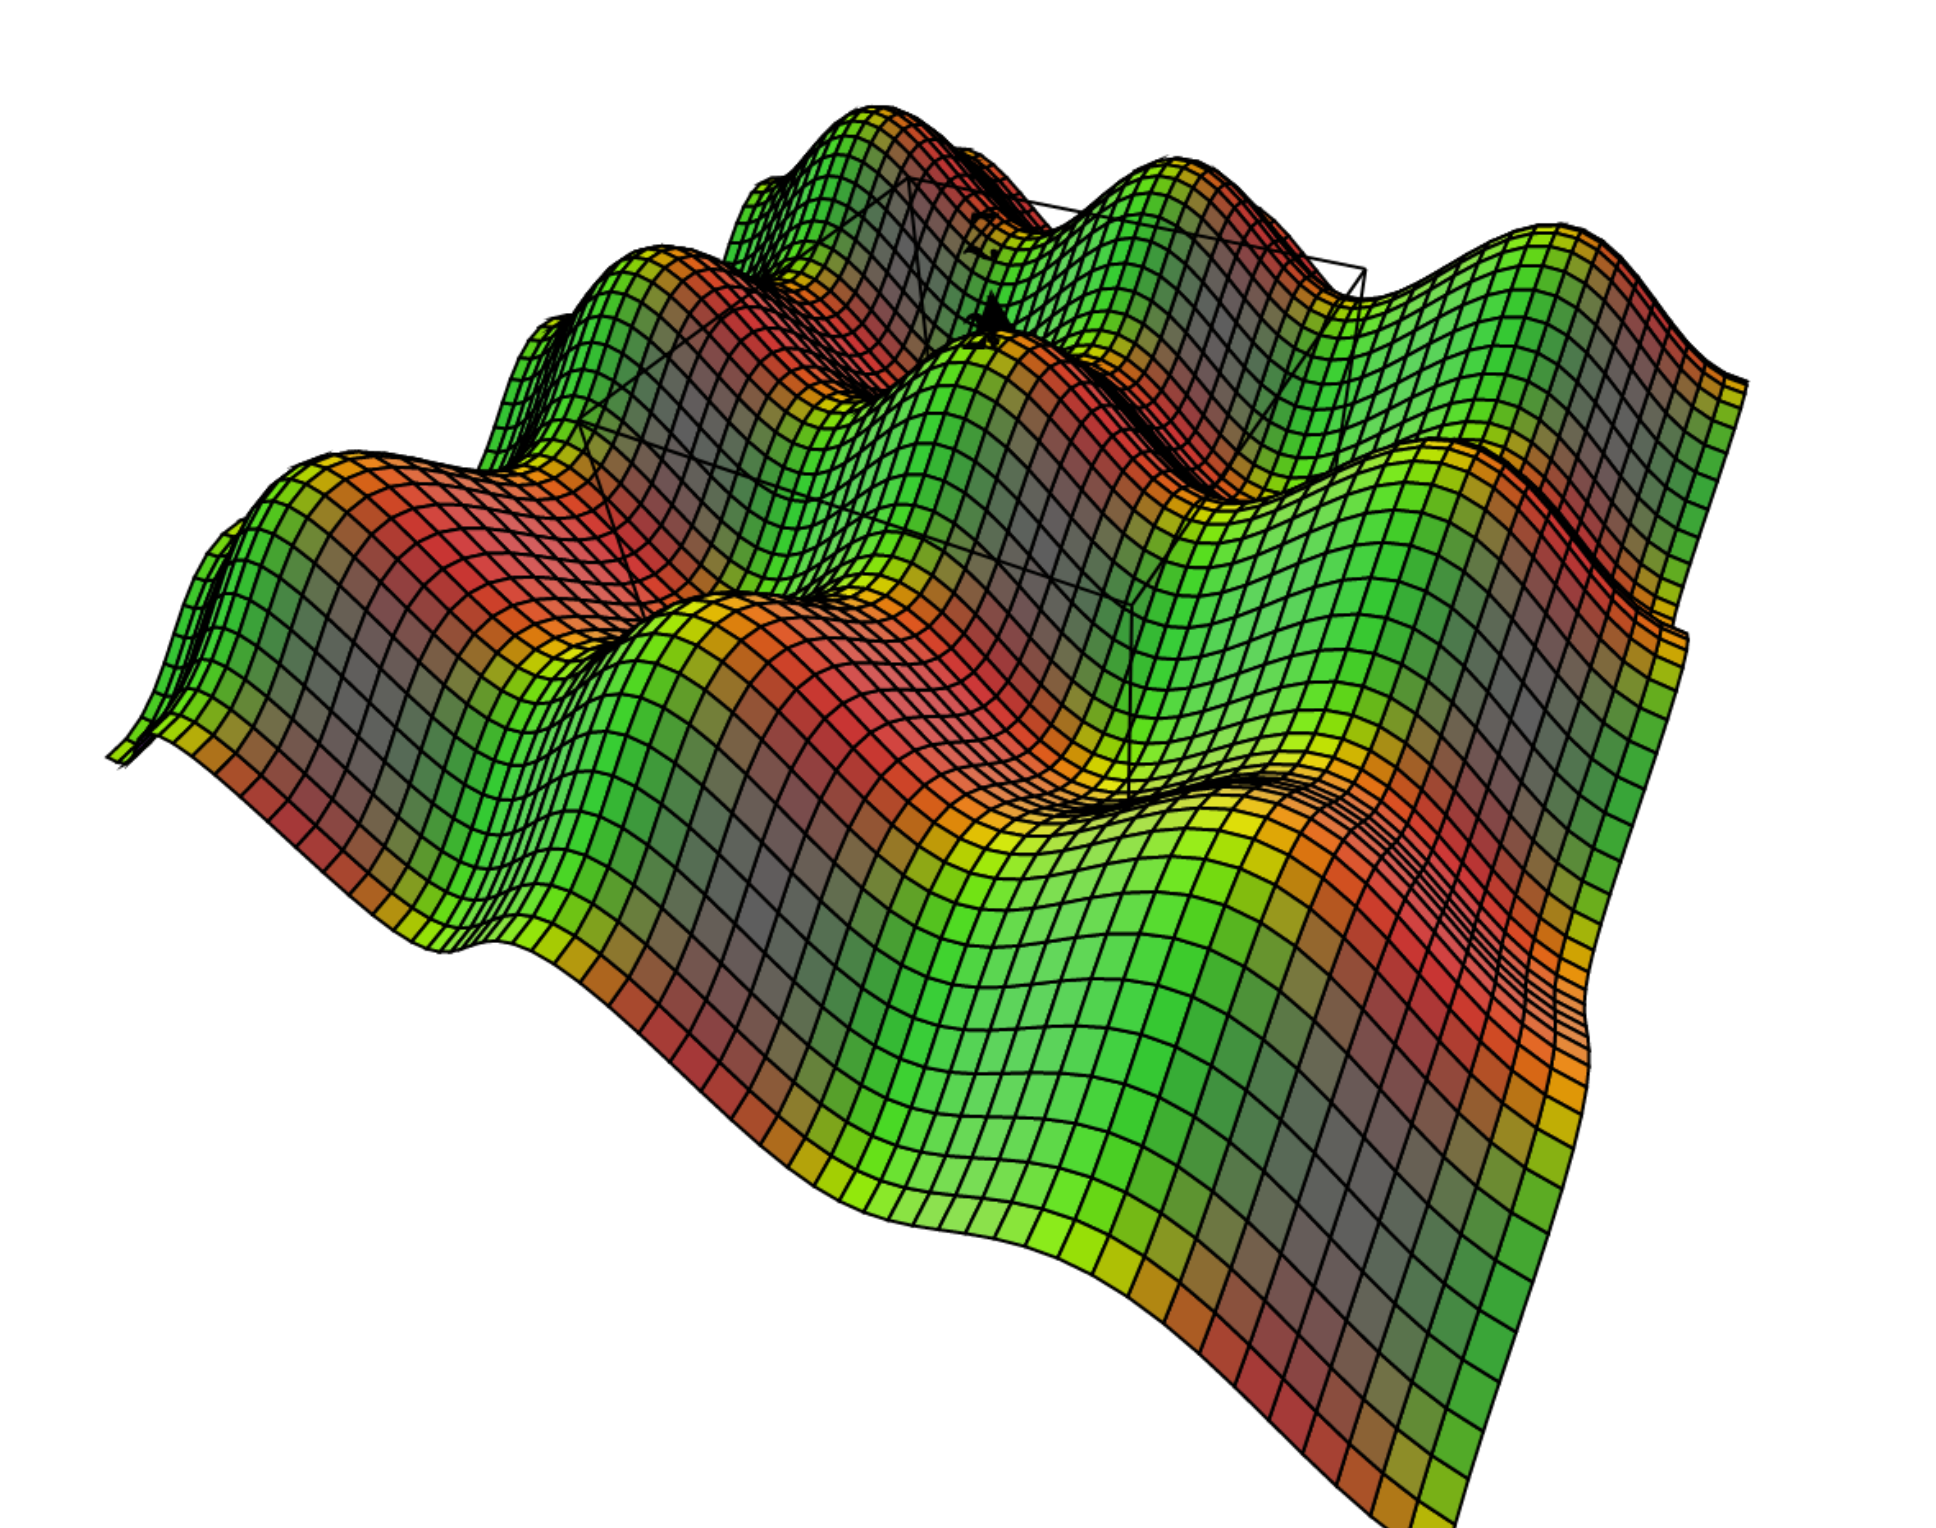
\includegraphics[width=.6\textwidth]{Images/crystal.png}
    \end{figure}
    
    \item Here is the plot of the level curves.
    \begin{figure}[H]
        \centering
        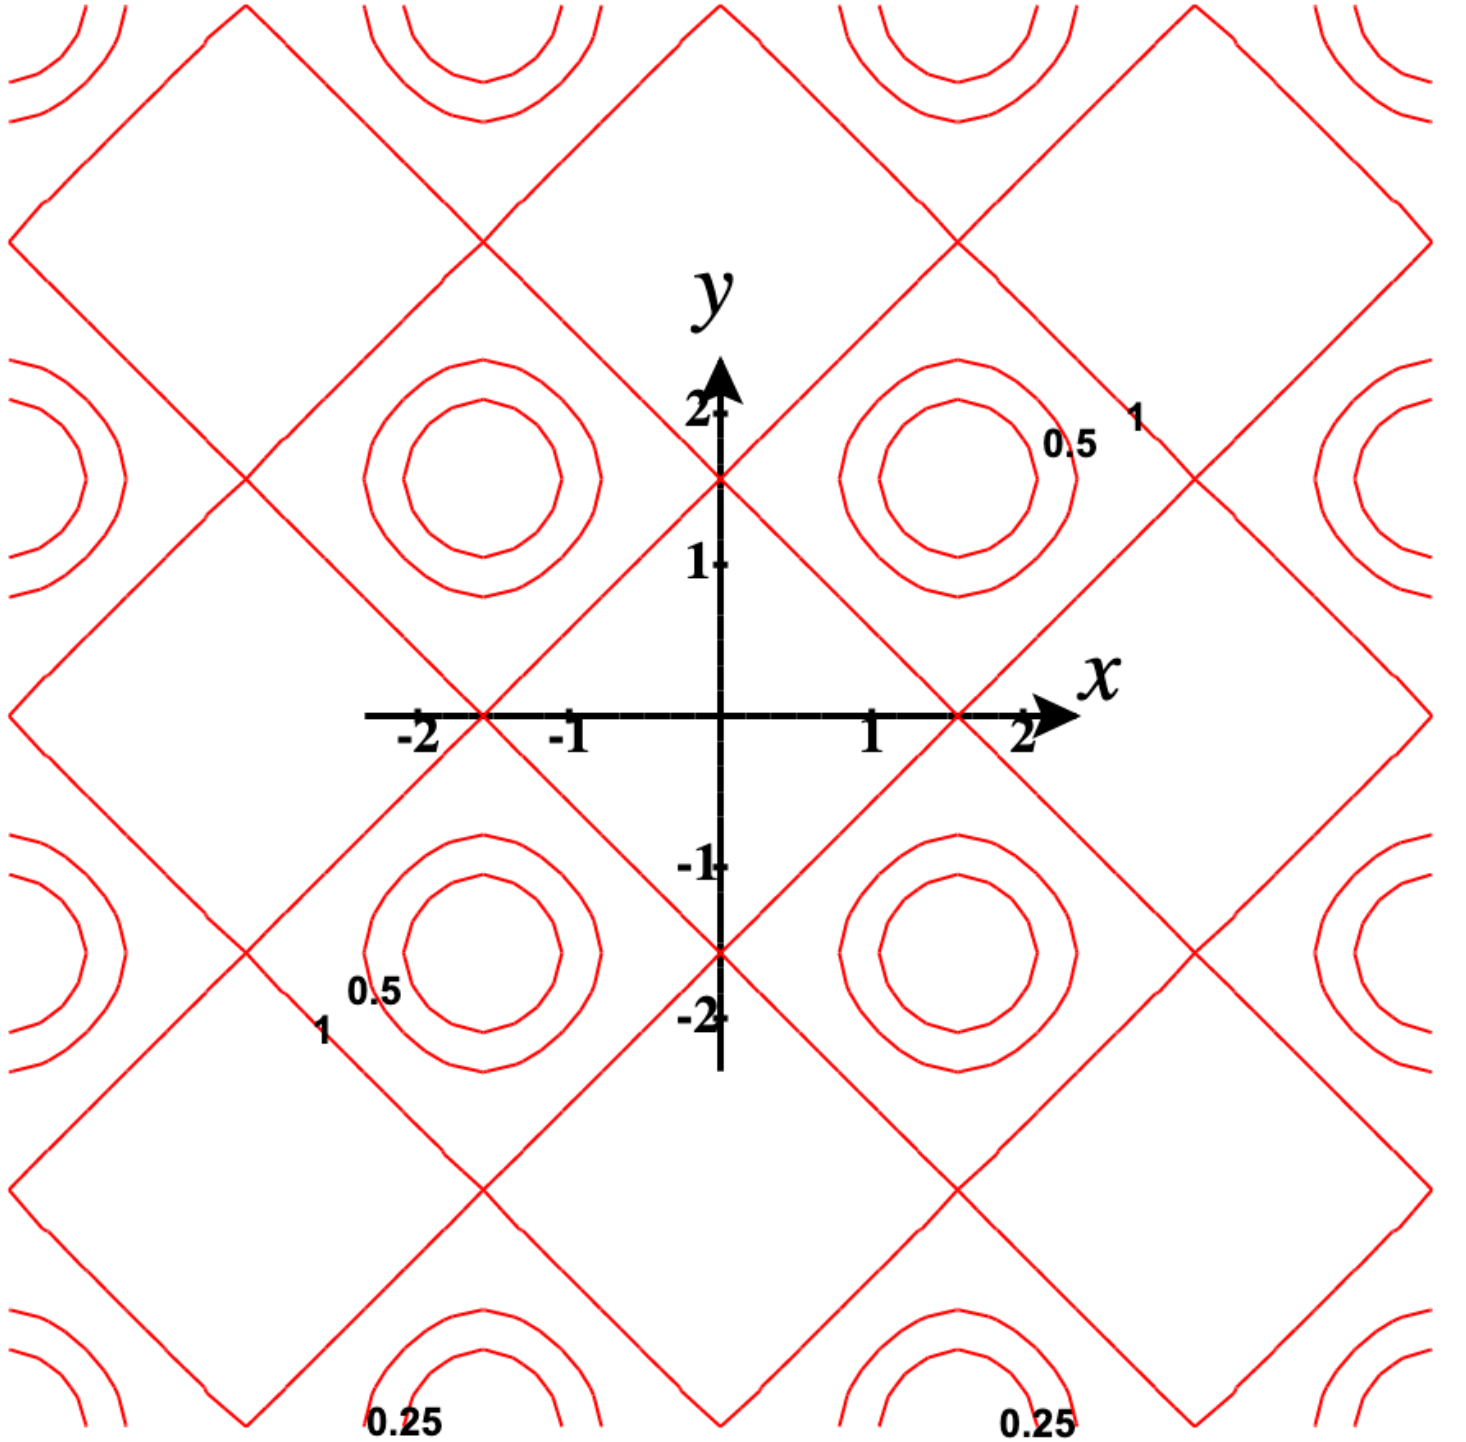
\includegraphics[width=.6\textwidth]{Images/crystal_contour.png}
        \caption{Smallest circles are $c=.25$, larger circles are $c=.5$, the lines are $c=1$ and $c=0$ are points in the centers of the squares and circles.}
        \label{fig:my_label}
    \end{figure}
    
    \item The gradient is
    \[
    \nabla u(x,y) = \begin{bmatrix} -2\cos(x)\sin(x) \\ -2\cos(y)\sin(y) \end{bmatrix}.
    \]
    \item We want to find where
    \[
    \nabla u(x,y) = \mathbf{0}.
    \]
    This gives us two equations to work with:
    \begin{align}
        -2\cos(x)\sin(x) &= 0,\\
        -2\cos(y)\sin(y) &= 0.
    \end{align}
    Note that (1) is zero whenever $\cos(x)$ or $\sin(x)$ is zero, which happens at $x=\frac{n\pi}{2}$ for all integers $n$. Similarly, we have that (2) is zero when $y=\frac{m\pi}{2}$ for all integers $m$.  This gives us many different solutions in our given range of values.
    
    If we think graphically, these values where the gradient is zero occur at the tops and bottoms of the peaks and valleys respectively.  These are the maxima and minima of the function $u(x,y)$.
    
    However, not all of these solutions are solutions where the electrons will want to stay put.  We will have to work harder to find out which ones are minimizers of the energy!
\end{enumerate}
\end{solution}


\noindent\textbf{Problem 4.} This function
\[
f(x,y)=\sin\left(\frac{2\pi x}{5}\right)\sin\left(\frac{2\pi y}{5}\right).
\]
comes up when you want to find out how a square shaped drum head will vibrate when hit. We'll see why later in the class, but for now do the following.
\begin{enumerate}[(a)]
    \item Plot this function on $0\leq x \leq 5$ and $0\leq y \leq 5$.  
    \item What can we say about the function $f(x,y)$ when $x=0$, $x=5$, $y=0$, and $y=5$?
    \item Compute $\frac{\partial^2 f}{\partial x^2}$, $\frac{\partial^2 f}{\partial y^2}$ and find $\frac{\partial^2 f}{\partial x^2}+\frac{\partial^2 f}{\partial y^2}$.
\end{enumerate}

\begin{solution}~
\begin{enumerate}[(a)]
    \item Here is the plot of the vibrating square drum head:
    \begin{figure}[H]
        \centering
        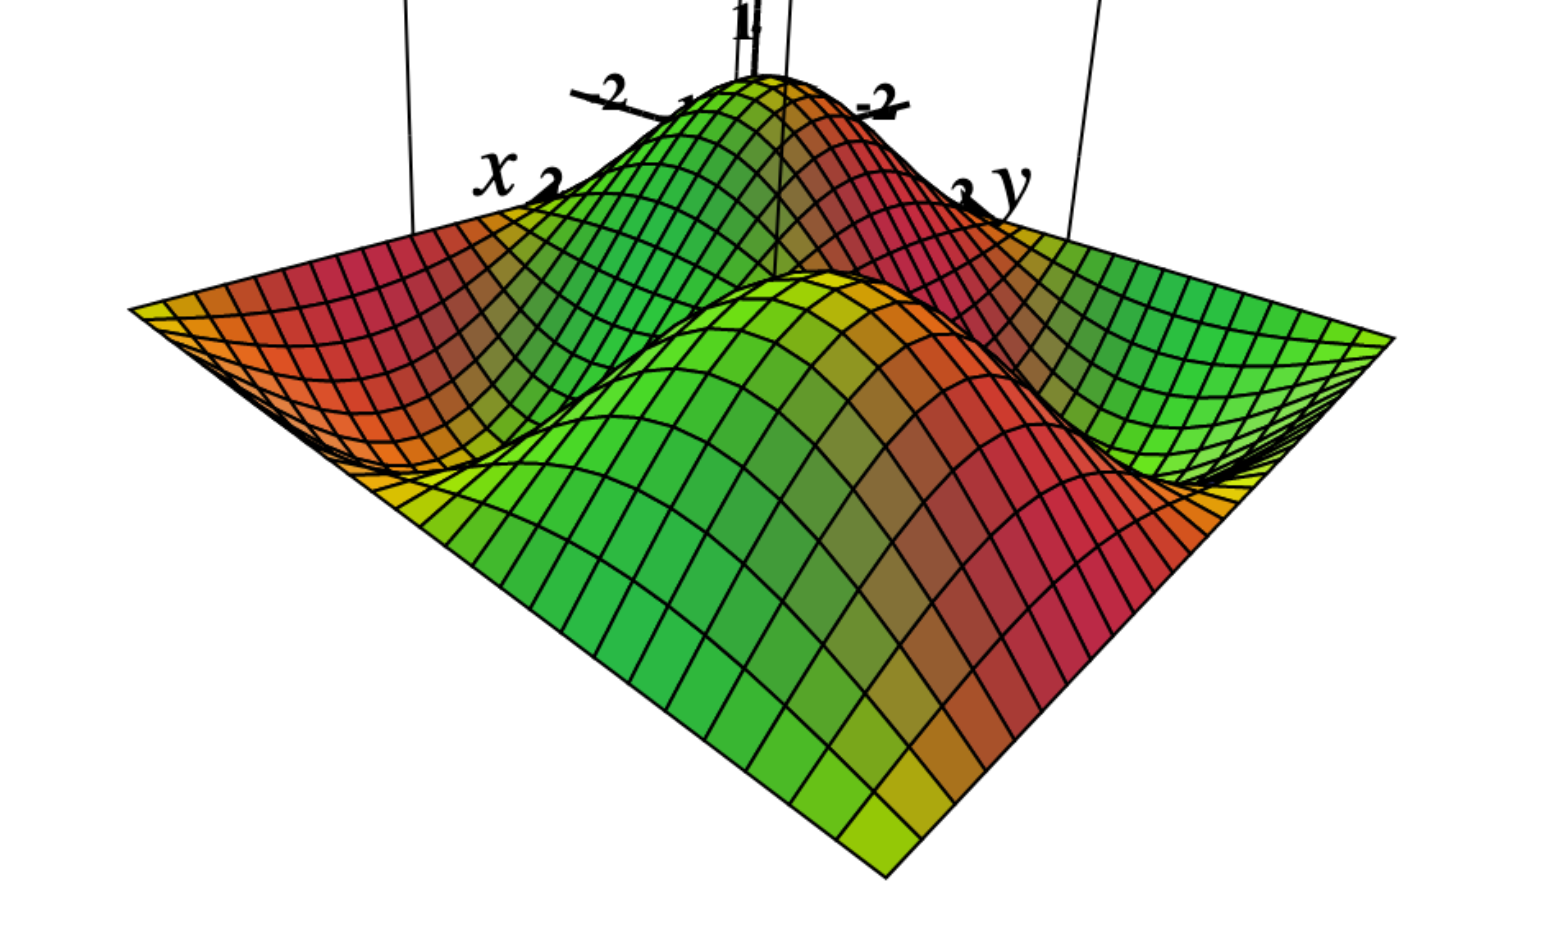
\includegraphics[width=.6\textwidth]{Images/square_drum.png}
    \end{figure}
    \item When $x=0$ we have
    \[
    f(0,y) = \sin\left( \frac{2\pi 0}{5}\right) \sin\left(\frac{2\pi y}{5}\right) = 0.
    \]
    Similarly, when $x=5$ $f(5,y)=0$, when $y=0$ $f(x,0)=0$, and when $y=5$ $f(x,5)=0$. 
    
    These are the boundary of the drum head.  That is, where the head of the drum is clamped down.
    
    \item We have
    \begin{align*}
        \frac{\partial f}{\partial x} &= \frac{2\pi}{5} \cos \left( \frac{2\pi x}{5} \right) \sin \left( \frac{2\pi y}{5} \right),\\
        \frac{\partial^2 f}{\partial x^2} &= \frac{-4\pi^2}{25} \sin \left( \frac{2\pi x}{5} \right) \sin \left( \frac{2\pi y}{5} \right),\\
        \frac{\partial f}{\partial y} &= \frac{2\pi}{5} \sin \left( \frac{2\pi x}{5} \right) \cos \left( \frac{2\pi y}{5} \right),\\
        \frac{\partial^2 f}{\partial y^2} &= \frac{-4\pi}{25} \sin \left( \frac{2\pi x}{5} \right) \sin \left( \frac{2\pi y}{5} \right).
    \end{align*}
    Then we have
    \[
    \frac{\partial^2 f}{\partial x^2} + \frac{\partial^2 f}{\partial y^2} = -\frac{8\pi^2}{25} \sin \left( \frac{2\pi x}{5} \right) \sin \left( \frac{2\pi y}{5} \right) = -\frac{8\pi^2}{25} f(x,y).
    \]
    The thing that's interesting is summing up these derivatives gives us back a multiple of our original function.  This feels eerily similar to the eigenvalue problem, because it is!  We haven't yet discussed the \emph{Laplacian} but the sum of these derivatives is the Laplacian in $2$-dimensions.  What we found here is that this function is an eigenfunction of the Laplacian! 
    
    So, the way a drum head vibrates is an eigen-problem, just with differential equations.
\end{enumerate}
\end{solution}

\noindent\textbf{Problem 5.} We have briefly discussed the idea of \emph{work} (think change in energy) before and wrote
\[
W=\mathbf{F}\cdot \mathbf{r}
\]
where $\mathbf{F}$ was a constant force and $\mathbf{r}$ was a straight line displacement.

Now we can write the real version of this.  The work done on a particle moving along a curve $\gamma(t)$ that starts at $t=t_0$ and ends at $t=t_1$ and experiencing a force $\mathbf{F}(x,y,z)$ is
\[
W=\int_\gamma \mathbf{F}(\gamma)\cdot d\gamma \coloneqq \int_{t_0}^{t_1} \mathbf{F}(\gamma(t))\cdot \gamma'(t) dt.
\]
Compute the work done given
\[
\mathbf{F}(x,y,z)=\begin{bmatrix} x^2\\ y\\ \sqrt{z}\end{bmatrix} \quad \gamma(t)=\begin{bmatrix} t\\ t^2\\t^3 \end{bmatrix} \quad t_0=0, ~ t_1=1.
\]

\begin{solution}
We have that
\[
\mathbf{F}(\gamma) = \begin{bmatrix} t^2 \\ t^2 \\ t^{3/2} \end{bmatrix}
\]
and
\[
\gamma'(t) = \begin{bmatrix} 1 \\ 2t \\ 3t^2 \end{bmatrix}.
\]
So we have
\begin{align*}
    W = \int_\gamma \mathbf{F}(\gamma)\cdot d\gamma &= \int_0^1 \begin{bmatrix} t^2 \\ t^2 \\ t^{3/2} \end{bmatrix} \cdot \begin{bmatrix} 1 \\ 2t\\ 3t^2 \end{bmatrix} dt\\
    &= \int_0^1 t^2 +2t^3+3t^{7/2}dt\\
    &= \left[ \frac{t^3}{3} + \frac{t^4}{2}+\frac{2t^{9/2}}{3}\right]_0^1\\
    &= \frac{3}{2}.
\end{align*}
\end{solution}




\end{document}  